\section{Input Impedance and Output Impedance}
\label{lab_input_output_impedance}

%\makelabheader %(Space for student name, etc., defined in master.tex)

\bigskip

\begin{enumerate}[wide]

\item Make a prediction for the voltage at the test point indicated in the circuit below.  Now build the circuit and test your prediction by measuring the voltage with your DMM.  Are you surprised?   \label{part_voltage_surprise}

\begin{center}
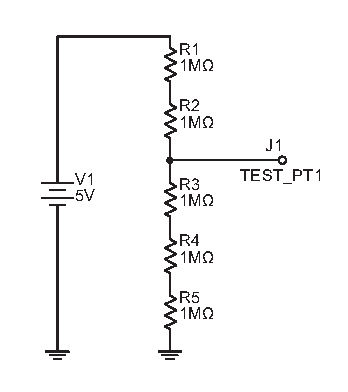
\includegraphics{input_output_impedance/input_impedance1.eps}
\end{center}

\item The reason for your surprise has to do with the input impedance of your voltmeter.  (For now, you can take the word ``impedance'' to be a synonym for ``resistance.''  In fact, you'll learn in lab \ref{lab_ac_circuits} that ``impedance'' is actually a little more general.)  What would be the input impedance of an ideal voltmeter?  What's the actual input impedance of your non-ideal DMM when it measures voltage?  (To find this out, you'll have to check in the manual for your DMM, under ``specifications''.) \label{part_dmm_impedance}

\item The internal resistance of your DMM can affect the circuit you are trying to measure.  To see how, consider the circuit at the right, which includes the actual input impedance of your DMM when it's used as a voltmeter.  Use the value of $R_{DMM}$ you found in part~\ref{part_dmm_impedance} to calculate the voltage at the test point in the figure below.  Does it agree with the voltage you measured in part~\ref{part_voltage_surprise}?

\begin{center}
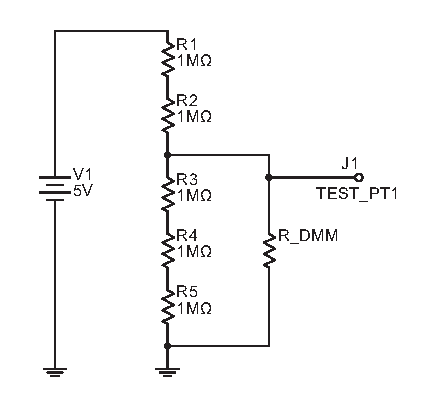
\includegraphics{input_output_impedance/input_impedance2.eps}
\end{center}

\item Make a prediction for the current through the 100~$\Omega$ resistor in the circuit below.  Now build the circuit and test your prediction by measuring the current with your red DMM, using its mA scale.  Are you surprised? \label{part_current_surprise}
 
\begin{center}

\includegraphics{input_output_impedance/current_measurement.eps}
\end{center}

\item The reason for your surprise (possibly less so than before) again has to do with the input impedance of your DMM.  What would be the input impedance of a (mythical) ideal current meter?  What's the actual input impedance of your DMM when it measures current?  Again, you'll have to check its manual.  They use the funny term ``burden voltage.''  (What are the units of that burden voltage, exactly?) \label{part_burden_voltage}

\item Again, the internal resistance of your DMM can affect the circuit you are trying to measure.  Use the value you reported in part~\ref{part_burden_voltage} to calculate the actual current through the 100~$\Omega$ resistor while you were measuring it with your DMM.  Does your result agree with what you measured in part~\ref{part_current_surprise}?

\item In this exercise, you will determine the internal resistance, or ``output impedance'' of your function generator.  Set your function generator to a large amplitude, 1~kHz sine wave.  

\begin{itemize}
\item First, use your DMM to measure the generator's AC output voltage when it is not hooked up to any load other than the DMM.  This is called its ``open circuit'' voltage.  

\item Next, use your DMM to measure the generator's AC output current when it is connected to ground through your DMM.  This is called the ``short circuit current''.   

\item Use the two measurements above to calculate the generator's internal resistance.  Compare your result to the output impedance listed in its instruction manual.
\end{itemize}

\item The short-circuit current measurement in the last part is okay for a relatively high impedance device like your function generator, but it is potentially dangerous for low impedance devices that can produce very large currents.  (Don't try short circuiting a car battery, for instance, or you could melt all your wires and cause the battery to explode!)  A safer method is to put a known load resistance $R_{LOAD}$ across the output terminals, and measure the voltage drop across $R_{LOAD}$.  By doing this, you have essentially made a voltage divider circuit using $R_{LOAD}$ and $R_{INTERNAL}$. Try this for your function generator, using a load resistance of $R_{LOAD} = 1$~k$\Omega$.  How do your results compare with the previous part? \label{part_func_gen_impedance}

\item Above, you used a load resistance slightly larger than your expected value for $R_{INTERNAL}$, which is generally a good choice.  How would your measurement be different if you had chosen  $R_{LOAD} = 100$~k$\Omega$, and how  would this affect how accurately you can determine $R_{INTERNAL}$?  Conversely, what would happen if you chose $R_{LOAD} = 1$~$\Omega$?  

\item When your DMM measures resistance, it does so by putting a small ``excitation current'' through the resistor and measuring the voltage.  How big is this excitation current?   (If it's not in the specifications, you could always measure it using another DMM….) 

\item Because the excitation current of the DMM is small, it's not very good at measuring resistances less than about an ohm.  Use your 5~V power supply in series with a 100~$\Omega$ resistor to put a larger ``excitation current'' through a single, long jumper wire on your breadboard, and measure the voltage across the wire to determine its resistance.  What's the smallest resistance you can reasonably measure this way?  Milliohms?  Micro ohms?  


\end{enumerate}


\textbf{Possible Exam Questions:}

\begin{itemize}
\item You have a 5~V source, and you would like to build a simple voltage divider using two equal resistors to give an output of 2.5 volts.  The 2.5 volt signal will go to an amplifier with an input impedance of about 50~k$\Omega$.  What value resistors should you use for your voltage divider: 1~k$\Omega$, 50~k$\Omega$, or 1~M$\Omega$?

\item You want to measure a current which you expect to be about 40~mA.  That amount of current can be measured using either the 400~mA range or the 10~A range.  What would be the advantage of using the 400~mA range?  What would be the advantage of using the 10~A range? (Yes, there is a specific advantage for each one.)  

\item From memory, what is the input impedance of your DMM when it is used as a voltmeter?  What is the input impedance of your DMM when it is used as an ammeter on the 10~mA scale?  On the 10~A scale?
\end{itemize}





